\documentclass[a4paper,11pt]{article}
\usepackage[utf8]{inputenc}
\usepackage[OT1]{fontenc}
\usepackage[english]{babel}
\usepackage[margin=1.2in]{geometry}
\usepackage{graphicx}
\usepackage{amsmath}
\usepackage{cite}
\usepackage[perpage,symbol]{footmisc}
\usepackage[hang,small]{caption}
%\usepackage{pslatex}

%\usepackage{fancyvrb}

\author{Simon Mitternacht}
\date{\today}
\title{Sasalib Manual}

\begin{document}
\maketitle
\hrule\vspace{0.5cm}
\noindent
The program/library Sasalib, including this manual, is licensed under
GPLv3, and can be downloaded from github at: 
\begin{center}
\texttt{https://github.com/mittinatten/sasalib/}
\end{center}
NB: This document is still a draft and not complete in any way.
\vspace{0.5cm}
\hrule
\section{Introduction}
The Solvent Accessible Surface Area (SASA) of a molecule gives a
measure of the surface of the molecule in contact with solvent. This
area can for example quantify how folded the conformation of a
macromolecule is, and can also be used to compare the exposed
hydrophobic surfaces of different conformations or different
molecules. To define the SASA, $A$, of given molecule, let a spherical
probe roll over the surface of the molecule, including internal
cavities. $A$ is then the surface drawn by the center of the
probe.~\cite{LnR} The probe represents a solvent molecule
(i.e.\ water), and therefore cavities that are too small for the
solvent to enter do not contribute to $A$.

Calculating Solvent Accessible Surface Areas (SASA) is a
run-of-the-mill type calculation in protein structure studies. To the
author's knowledge there are no fully open source standalone programs
for doing this. Neither are there any libraries designed to be easily
integrated in other programs. The present library is an attempt to
resolve both these issues, and is released under the GNU General
Public License 3.0.

Sasalib is a both a standalone command line program and a C library
for protein SASA calculations. The library provides a simple interface
that takes PDB-files as input. It has default parameters to allow
straightforward calculations, but also allows the user to change most
parameters of the calculation. In addition, there is a lower level
interface where the user can treat the calculation as a purely
mathematical operation on a set of spheres, specifying only
coordinates and radii. Both Lee \& Richards' \cite{LnR} and Shrake \&
Rupley's \cite{SnR} algorithms are available. They will be referred to
as L\&R and S\&R throughout this document. Future versions of the
library might include other algorithms as well.

In constructing the library three possible use cases were considered. 
\begin{enumerate}
\item The user has a PDB-file and wishes to calculate total SASA of
  the structure, or the SASA for certain groups or types of atoms.
\item The user has a set of cartesian coordinates for atoms and radii
  for these atoms and wants to calculate the total SASA for this object. 
\item The user is simulating a molecule and wants to sample SASA of
  different configurations during the simulation.
\end{enumerate}
For case 1 both the command-line interface (CLI) and the application
programming interface (API) can be used. Using the API gives more
flexibility in interpreting and analyzing the results. The other 2
cases can only be handled through the API. Both the API and the CLI
allow the user to set parameters for the calculation. 

This document is organized as follows. Section \ref{sec:howto_short}
give a brief introduction to the library, presenting the command line
interface and a short sample program that gives a general idea of how
to use the library. Section \ref{sec:alg} describes the algorithms and
compares their performance in terms of computational cost and
precision. In section \ref{sec:imp} the implementations are
described. Finally, section \ref{sec:using} gives a detailed
description of the library interface.

\section{Getting started}\label{sec:howto_short}

The source files \texttt{calc\_sasa.c} and \texttt{example.c} contain
a complete command-line interface and a minimal program to illustrate
how to use the library interface, respectively. 

\subsection{Installation} \label{sec:installing}

The repository can be cloned from github, either by using git directly
with the command
\begin{verbatim}
    $ git clone https://github.com/mittinatten/sasalib.git
\end{verbatim}
or by downloading the zipped archive from
\begin{verbatim}
    https://github.com/mittinatten/sasalib/archive/master.zip
\end{verbatim}
Since Sasalib only depends on regular C and GNU libraries most users
will be able to compile it by simply typing \texttt{make}\footnote{Has
  been tested on Linux and Mac OS X machines.}. If any compiler other
than the Gnu C Compiler is preferred the makefile will need to be
changed accordingly. The command \texttt{make example} compiles the
example program described in section \ref{sec:simple_sample}.

\subsection{Command-line interface}

Compilation creates the binary \texttt{calc\_sasa} from
\texttt{calc\_sasa.c}, which can be used to calculate the SASA of a
PDB-file. The simplest program call, with default parameters would be
\begin{verbatim}
    $ ./calc_sasa PDB-file
\end{verbatim}
Or, from STDIN:
\begin{verbatim} 
    $ ./calc_sasa < PDB-file    
\end{verbatim}
STDIN is only read if no file is specified.  By default the Shrake \&
Rupley algorithm is used, with 100 test points. Section \ref{sec:CLI}
shows how to specify algorithm and parameters. For a quick look at
command-line options, use the command
\begin{verbatim}
    $ ./calc_sasa -h
\end{verbatim}
Running the program using the default parameters on the PDB structure
1UBQ gives the following output
\begin{verbatim}
    name: [path to pdb-files]/1ubq.pdb
    algorithm: Shrake & Rupley
    n_thread: 1
    n_testpoint: 100
    time_elapsed: 0.019065 s
    n_atoms: 602

    Total:   4756.12 Å2
    Polar:   1968.06 Å2
    Apolar:   2788.07 Å2
\end{verbatim}
The first 4 lines contain info about input and parameters. This is
followed by data over calculation time and the size of the
protein. Finally the result of the calculation is printed, with SASA
values in Å$^2$.

\subsection{Simple example (\texttt{example.c})}\label{sec:simple_sample}

The following shows the minimal program \texttt{example.c} that
performs a SASA-calculation using a PDB-file as input. This program is
basically a stripped down version of \texttt{calc\_sasa.c} without
error handling, and without any commandline options. This code is
meant to illustrate the most basic parts of the library interface.
\begin{verbatim}
#include <stdlib.h>
#include "src/sasalib.h"

int main(int argc, char **argv) { 
    //initialize sasalib-object with default parameters
    sasalib_t *s = sasalib_init();

    //do the calculation using default parameters with protein
    //structure from STDIN
    sasalib_calc_pdb(s,stdin);

    //print results
    sasalib_log(stdout,s);
    printf("Total area: %f Å2\n", sasalib_area_total(s));

    //clean up
    sasalib_free(s);

    return EXIT_SUCCESS;
}
\end{verbatim}
This program generates results similar to that in the previous
section.

\section{Algorithms}\label{sec:alg}

There are two classical approximate algorithms that can be used to
calculate SASA, by Lee \& Richards \cite{LnR} and Shrake \& Rupley
\cite{SnR} respectively. Both can be calculated to arbitrary precision
by refining the resolution. 

As will be clear from this section and the analysis in section
\ref{sec:compare}, S\&R is the simpler and faster of the
two. Therefore the casual user is recommended to use S\&R. L\&R is
mainly included for reference, and for the fact that the precision is
only limited by floating point precision. In the current
implementation S\&R can only be used with a predefined set of levels
of precision. However, since SASA is not a fundamental measure or
concept, it is not obvious what applications would require very high
precision.

We will use the following notation: An atom $i$ has a van der Waals
radius $r_i$, the rolling sphere (or \emph{probe}) has radius
$r_\text{P}$ and when these are added we get $R_i = r_i +
r_\text{P}$. The SASA for a molecule is then obtained by calculating
the non-buried surface area of all the individual spheres with radius
$R_i$ atom and adding them up.

\subsection{L\&R} \label{sec:alg_LnR}

Lee \& Richards' algorithm calculates the surface area by slicing the
protein, calculating the length of the solvent exposed contours in
each slice and then adding up the length multiplied by the slice
thickness. Precision is increased by making the slices thinner and the
calculation time scales approximately as the number of slices.

Divide the protein into slices of thickness $\delta$ along an
arbitrary axis. The position of the slice along that axis is denoted
$z$. The center of atom $i$, along the same axis, is at $z_i$. In the
slice, each atom is thus a circle of radius $$R_i^\prime =
\sqrt{R_i^2-(z-z_i)^2}\,.$$ These circles are either completely
buried, completely exposed, or partially exposed.

The exposed arc lengths for each atom can be calculated exactly. For
each pair of atoms $i,j$, the distance between their centers projected
on the slice is $d_{ij}$ (independent of $z$). If $d_{ij} > R_i^\prime
+ R_j^\prime$, there is no overlap. If $d_{ij} < R_j^\prime -
R_i^\prime$ circle $i$ is completely inside $j$ (and the other way
around). If $d_{ij}$ lies between these two cases the angle of circle
$i$ that is buried due to circle $j$ is $$\alpha = 2\arccos
\bigl[({R_i^\prime}^2 + d_{ij}^2 - {R_{j}^\prime}^2)/(2R_i^\prime
  d_{ij})\bigr].$$ The middle point of the arc on the circle is at an
angle $\beta$ in circle $i$, and thus the arc spans the interval
$[\beta-\alpha/2,\beta+\alpha/2]$ on the circle. By adding up these
arcs and taking into account any overlap between them we get the total
buried angle $\gamma_i$ of circle $i$. The exposed arc length in this
slice is thus $L_i = R_i^\prime(2\pi-\gamma_i)$.

The contribution to the SASA from each slice is $$ S_\delta =
\sum_{i \in \text{slice}}L_i\Delta_i $$ where
$$
  \Delta_i = \frac{R_i}{R_i^\prime} \biggl[\frac{\delta}{2} 
    + \min\biggl(\frac{\delta}{2},R_i -
    \lvert z - z_i \rvert\biggr)\biggr]. 
$$ 
The factor $R_i/R_i^\prime$ comes from approximating the area by a
conical segment tangent to the sphere in the slice, instead of a
cylinder.  Finally, the total SASA is obtained by adding up the
contribution from all the slices, either for the whole protein, or
atom by atom.

\subsection{S\&R}

For each atom $i$, use a set of test points evenly distributed
(approximately) over the sphere of radius $R_i$, and count how many of
the test points are not inside any of the other extended spheres of
radius $R_j$. The number of exposed test points divided by the total
number of test points gives the exposed solid angle of that atom. The
precision of the algorithm is increased by increasing the number of
test points, and calculation time scales approximately linearly with
the number of test points.


\section{Implementation}\label{sec:imp}

This section describes the implementation of the algorithms in general
terms. In both cases the implementations are rather straightforward,
to make them simple and transparent. See sections
\ref{sec:howto_short} and \ref{sec:using} for instructions for how to
install and use the library.

The implementations were tested by performing high precision SASA
calculations using both algorithms for a large number of proteins (see
section \ref{sec:dataset}) and comparing the results. Also, the
calculated surface test points and slice contours were verified by
visual inspection.

\subsection{L\&R}

The L\&R-calculation needs to know which atoms make contacts for each
slice. Therefore the calculation begins by constructing adjacency
lists for the protein. An contact matrix was used in early versions of
the library, but the $O(N^2)$ memory requirements were prohibitive for
large proteins. For each slice the adjacency lists are condensed to
separate lists only containing the atoms in that particular
slice. Each pair of adjacent atoms is then checked for adjacency in
the particular slice and the overlapping arcs are calculated as
described in section \ref{sec:alg_LnR}. When all buried arcs are
counted for a given atom they are reduced to non-overlapping intervals
recursively. In most cases this is done in one step, sometimes in two
or three. The arc-lengths are then summed up for all atoms in the
slice to calculate the total contribution to the area as described in
\ref{sec:alg_LnR}.

As described in section \ref{sec:accuracy}, this algorithm is
significantly slower than S\&R. Profiling runs give no hints at
obvious improvements. The calculations of each slice are however
completely independent and the current implementation allows division
of labor to an arbitrary number of threads. The $O(N^2)$ calculation
of adjacency lists has not been parallelized in the current
implementation. The calculation could be both linearized and
parallelized by using cell lists, but since the adjacency lists are
only calculated once for each protein the overhead of setting up the
cell lists is likely to be prohibitive for all but the largest
proteins.\footnote{A preliminary, somewhat buggy implementation of
  cell lists verified that at least linearization alone was not worth
  the effort. Might be worth investigating how it performs in
  parallel.}


\subsection{S\&R}

In S\&R the list of neighbors for each atom is only used once, hence
it is not precalculated. Generally the cost of calculating overlap
between two spheres is much larger than identifying which atoms are
neighbors, except in the case of very few test points. Calculating
atom contacts on the fly also allows trivial parallelization of the
whole calculation.

Test points were generated by placing a given number of equally
charged particles on the surface of a sphere and then minimizing the
Coulomb potential using a simple Monte Carlo simulation. The obtained
sets of test-points are then stored as static arrays in a special
source file (\texttt{srp.c}), to make the program independent of any
auxiliary input files. Sets containing 20, 50, 100, 200, 500, 1000,
2000 and 5000 test points are included in the program. This set should
cover most users' need for speed and accuracy.

\subsection{Comparison of the two}\label{sec:compare}

\subsubsection{Data set}\label{sec:dataset}

For evaluating and comparing the two algorithms a list of proteins was
downloaded from the PISCES server (on Aug 12, 2013). The proteins have
less than 20\,\% sequence identity, and the structures a resolution of
1.6~Å or less and R-factors less than 0.25\footnote{The resolution of
  the structures is not relevant for the present study. It was only
  restricted to get a sufficiently small set of independent
  structures.}. The list specifies which chain to use in a specific
PDB-file. For the calculations here, whole PDB-files are used, giving
a larger variation in protein size, which is useful for our
purposes. The 2117 chains in the list gave a set of 2056 protein
structures used for all calculations below.

\subsubsection{Speed}

In the limit of low precision the calculation time will be limited by
the time it takes to find which atoms are neighbors, which scales as
the square of the number of atoms. As described above this calculation
can be linearized, but with a relatively large overhead making it
worthwhile only for large proteins.

In the limit of high precision the calculation time of both algorithms
will instead scale as the number of atoms: If the number of
test-points is large in S\&R, most of the time will be spent
calculating the extent of overlap, instead of which atoms are in
contact. If there are many slices in L\&R, the calculation time will
be proportional to the number of slices, and the time of each slice
linear in the number of atoms in the slice.  The point where the
calculation time crosses over from linear to quadratic in the number
of atoms thus depends on the precision as figure~\ref{fig:time} shows.

\begin{figure}
  \begin{center}
  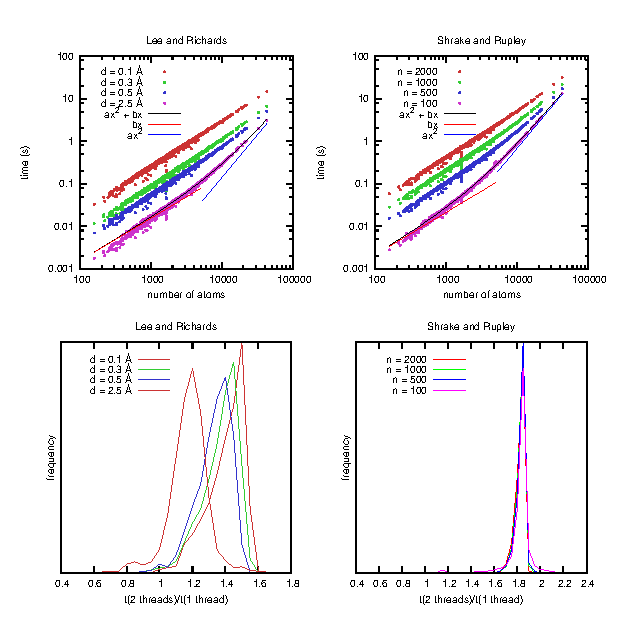
\includegraphics{../analysis/plots/time}
  \caption{(Top) Calculation time as function of number of atoms for
    different levels of precision. In both cases the cross-over from
    linear to quadratic scaling as function of protein size is only
    clearly visible for the lowest precision used.  (Bottom)
    Comparison of calculation time with one and two threads, the
    histograms shows the distribution of the calculation time using
    two threads divided by the time using one thread. Thus a value of
    2 would correspond to ``perfect'' parallelization. The values
    above 2 are likely due to noise, i.e. in the very short
    simulations the timing is both inexact and might be affected by
    random factors such as background system processes.
    \label{fig:time}}
  \end{center}
\end{figure}

Where it can be done trivially, both algorithms have been
parallelized. As mentioned above, in S\&R each atom can be treated
independently, and in L\&R each slice. The efficiency of the
parallelization in a two-threaded run can be seen in figure
\ref{fig:time}. For S\&R the speed increase is close to twofold and
independent of the accuracy, as expected. For L\&R the efficiency of
parallelization increases with precision, i.e. the more slices are
calculated, the more there is to gain from parallelizing the
calculations. This result was also expected since the time needed to
compute which atoms are neighbors, which is done in only one thread in
the current implement, is independent of precision.

\subsubsection{Accuracy as function of speed}\label{sec:accuracy}

To measure accuracy of the two algorithms a reference SASA value,
$S_\text{ref}$ was calculated using L\&R with slice thickness
0.001~Å. The error of a given SASA-value, $S$ is then $\delta = \lvert
S - S_\text{ref} \rvert / N$, where $N$ is the number of atoms in the
protein. Figure~\ref{fig:precision} shows the results of these
calculations for the 2056 proteins described above.  It is clear from
this picture that S\&R is on average an order of magnitude more
accurate than L\&R given the same computational effort -- in the
present implementation.

\begin{figure}
  \begin{center}
  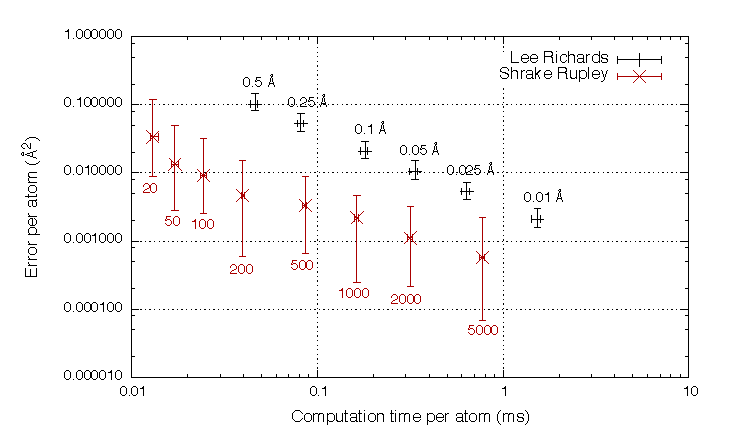
\includegraphics{../analysis/plots/precision}
  \caption{The error $\delta$ in calculated SASA vs calculation time
    $t$ for the two algorithms. For the different S\&R calculations
    20, 50, 100, 200, 500, 1000, 2000 and 5000 test points were
    used. For L\&R slice thicknesses 0.01, 0.1, 0.2, 0.3, 0.5, 1.0,
    2.5 and 5.0 Å. The borders of the boxes indicate the quartiles of
    the distribution of $t$ and $\delta$ (i.e. 50~\% of the data are
    within the box), and the error bars 5th and 95th percentiles.
    \emph{Why is S\&R distribution much wider?}
    \label{fig:precision}}
  \end{center}
\end{figure}



\section{Using Sasalib} \label{sec:using}

\subsection{Command line interface}\label{sec:CLI}

\subsection{Library interface}

Sasalib has two levels of library interface. The simplest interface
assumes the user does not want to access the results in any raw form
and takes care of most of the allocation of resources. This
functionality is specified in the header \texttt{sasalib.h}. The
sample program in section \ref{sec:simple_sample} uses this interface.
In addition to what is shown in the example this interface also allows
setting user settings. This is documented in the header, and the program
\texttt{calc\_sasa.c} illustrates how this can be used.

To gain data access to atom-per-atom data, to specify custom radii or
to define one's own groups of atoms to calculate SASA over, a deeper
level is also available. The library mainly provides functions for
doing the following in different ways
\begin{enumerate}
  \item Initialize protein.
  \item Calculate atomic radii.
  \item Calculate SASA.
  \item Output results grouping atoms/residues in different ways.
\end{enumerate}
The third step is the core functionality of the library and can be
used separately if users wish to handle the other steps
themselves. Below follows a brief description for the functionality
provided for each of the four steps, but first a sample program
showing a complete workflow.

\subsubsection{Sample program using low-level interface}
The following lines read a PDB-structure from a file, calculates
SASA using Lee \& Richards' algorithm and outputs the values for the
polar and apolar atoms respectively.
\begin{verbatim}
#include <stdio.h>
#include <stdlib.h>
#include "src/protein.h"
#include "src/sasa.h"

int main(int argc, char **argv) {
    // initialization from STDIN
    protein *p = protein_init_from_pdb(stdin);

    // allocate memory
    double *sasa = (double*) malloc(sizeof(double)*protein_n(p));
    double *r = (double*) malloc(sizeof(double)*protein_n(p));

    // calculate atomic radii
    protein_r_def(p,r);
    
    // SASA calculation using Lee & Richards with 
    // slices of width 0.25 Å
    sasa_lee_richards(sasa,protein_xyz(p),r,protein_n(p),0.25);

    // Output SASA for polar/apolar atoms
    sasa_per_atomclass(stdout,oons_classes(),p,sasa);
   
    // free memory
    protein_free(p);
    free(sasa);
    free(r);

    return 0;
}
\end{verbatim}

\subsubsection{Initiate a protein}

A protein is represented by the struct \texttt{protein}, which is
declared in the header \texttt{protein.h}. A proteins can be
initialized either by reading a PDB-file or by adding atoms manually
one-by-one.

The following function initializes a protein from a PDB-file
\begin{verbatim}
    protein* protein_init_from_pdb(FILE*); 
\end{verbatim}
The pointer is freed using
\begin{verbatim}
    void protein_free(protein*);
\end{verbatim}
An empty protein struct is allocated with 
\begin{verbatim}
    protein* protein_init();
\end{verbatim}
which can then be used to add atoms one by one
\begin{verbatim}
    void protein_add_atom(protein *p, 
                          const char* atom_name,
                          const char* residue_name, 
                          const char* residue_number,
                          char chain_label,
                          double x, double y, double z);

\end{verbatim}
for example like this
\begin{verbatim}
    protein *p = protein_init();
    protein_add_atom(p, " CA ", "GLY", "   1", "A",
                     x, y, z);
\end{verbatim}
Here the labels for the atom are as they would be in a PDB file,
including whitespace. The atom name is a 4-character string, like the
second argument above, the residue name a 3-character string, like the
third argument, the residue number has 4 characters, and the chain
label 1. The last three arguments are the coordinates of the atom. The
reason residue numbers are not represented as integers here, is that
some PDB files have number sequences such as 1A, 1B, 1C, 1D, 2, 3, 4,
\ldots.

The rationale for directly using the strings found in PDB files is
twofold. (i) Most programs that handle proteins will have routines for
generating PDB-files and it should thus be fairly straightforward to
integrate this library into such a program. (ii) Non-standard atoms
can be added with the labels they have in the input, making
sub-sequent analysis more straightforward. This means that no analysis
is performed of the atom types, to check for consistency, etc. The
atom types are only used later for assigning radii to the atoms,
something that can also be done manually.

\subsubsection{Assign atomic radii}
Give each atom a radius. Sasalib can calculate atomic radii according
to Ooi et al (OONS-radii) for the 20 canonical amino acid types. The
user can also specify the radius for each individual atom. The two
methods can be combined if a protein has a few non-standard atoms.

Functions for OONS-classification are found in \texttt{oons.h}. There
are two versions
\begin{verbatim}
    double oons_radius_pdbline(const char *pdb_line);
    double oons_radius(const char *res_name,
                       const char *atom_name);
\end{verbatim}
where the argument in the first version is a line from a PDB-file, and
in the second case residue name and atom name according to the above
(e.g. \texttt{"GLY", " CA "}). To get all radii for a protein in one
go, use
\begin{verbatim}
    void protein_r_def(double *r, const protein *p);
\end{verbatim} 
Here the array \texttt{r} is assumed to be of the same size as the
protein, i.e. the user is responsible for allocating and freeing the
memory. The function
\begin{verbatim}
    int protein_n(const protein *p);
\end{verbatim}
returns the number of atoms in a protein.  A user-defined
atom-classification scheme can be used by calling
\begin{verbatim}
    void protein_r(double *r,
                   const protein *p, 
                   double (*atom2radius)(const char *res_name, 
                                         const char *atom_name));
\end{verbatim}
The function \texttt{protein\_r\_def}, defined above, uses
\texttt{protein\_r} internally. It consists of the single line
\begin{verbatim}
    protein_r(p,r,oons_radius);
\end{verbatim}
which illustrates the use of the functions \texttt{protein\_r} and
\texttt{oons\_radius}.

\subsubsection{Perform SASA calculations}
Perform the SASA calculation, using the algorithm of choice, calling
the functions in \texttt{sasa.h}
\begin{verbatim}
    void sasa_shrake_rupley(double *sasa,
                            const vector3 *xyz,
                            const double *radii,
                            size_t n_atoms,
                            int n_points);
    void sasa_lee_richards(double* sasa,
                           const vector3 *xyz,
                           const double *radii,
                           size_t n_atoms,
                           double grid);

\end{verbatim}
The protein struct is deliberately not used here to allow users to
only use this function independently of the rest of library. The
header \texttt{vector3.h} provides an interface to generate arrays of
type \texttt{vector3} for the coordinates from either three arrays of
\texttt{double}s of size $N$ using the function
\texttt{vector3\_xyz\_alloc()}, or one array of size $3N$ where the
coordinates are arranged $x_1,y_1,z_1,x_2,y_2,z_2,\ldots,x_N,y_N,z_N$
using the function \texttt{vector3\_x3n\_alloc()}. The generated array
can then be used as input for the two functions above.

\subsubsection{Output results}
The header \texttt{atomclassifier.h} specifies an interface for
classifying atoms in a protein. The struct \texttt{atomclassifier} has
a function pointer to a function that turns a residue- and atom-name
to an integer, and an array of strings that explains what these
integers means. The function \texttt{atomclassifier\_all()} returns an
\texttt{atomclassifier} object that puts all atoms in the same class,
which can be used to calculate the total SASA of a protein. The header
\texttt{oons.h} has functions to generate two types of
\texttt{atomclassifier}s. One that returns an \texttt{atomclassifier}
for polar/apolar atoms, and another for the classes aliphatic C,
aromatic C, hydroxyl O, etc (as specified in reference \cite{OONS}),
respectively. Users interested in implementing their own classifiers
can use the source for these functions as an illustration.

In \texttt{sasa.h}, the function
\begin{verbatim}
    void sasa_per_atomclass(FILE*, atomclassifier, 
                            protein*, double *sasa);
\end{verbatim}
integrates the results of the SASA calculation using an
\texttt{atomclassifier} to get for example the polar and apolar
surface areas. The statement
\begin{verbatim}
    sasa_per_atomclass(stdout, oons_classes(),p,s);
\end{verbatim}
where \texttt{p} is a pointer to a \texttt{protein} object, and
\texttt{s} an array of appropriate size containing SASA values for the
atoms of the protein, will output the following
\begin{verbatim}
    > polar_apolar
    polar 1234.56
    apolar 7890.12 
\end{verbatim}
That is the name of classifier, and the SASA values for each class of
atoms, in this cased the two classes \emph{polar} and \emph{apolar}.

\section{Known issues}

The atoms of non-standard amino acids will be labeled unknown type,
and their contribution to for example the polar/apolar area will have
to be integrated manually by the user.

\section{Ideas for improvement and extension}

In no specific order
\begin{itemize}
\item Perl and Python bindings.
\item Other, faster or more exact algorithms.
\item Molecular surface calculations?
\item Add a library of commonly seen non-standard atoms, such as those
  in capping end groups and in phosphorylated amino acids.
\item Interface to download PDB-file and calculate SASA given only PDB
  code.
\end{itemize}

\begin{thebibliography}{50}

\bibitem{LnR} 
  Lee B, Richards FM (1971) The interpretation of protein
  structures: estimation of static accessibility. Journal of molecular
  biology 55: 379–-400.

\bibitem{SnR} 
  Shrake A, Rupley JA (1973) Environment and exposure to
  solvent of protein atoms. Lysozyme and insulin. Journal of Molecular
  Biology 79: 351–-371.

\bibitem{OONS} 
  Ooi T, Oobatake M, Némethy G, Scheraga H (1987)
  Accessible surface areas as a measure of the thermodynamic
  parameters of hydration of peptides. Proceedings of the National
  Academy of Sciences of the United States of America 84: 3086–3090.

\bibitem{PISCES}
  Wang G, Dunbrack RL (2003) PISCES: a protein sequence culling server. 
  Bioinformatics 19:1589--1591.

\end{thebibliography}

\end{document}
